\documentclass[12pt]{ctexart}
\usepackage{amsmath,graphicx,textcomp,subfigure,indentfirst,ctex,color,float}
\title{Lecture 7}
\author{赵思逸}

\date{2022年4月12日}

\newcommand{\refeq}[1]{式~(\ref{#1})}
\newcommand{\reffig}[1]{图~(\ref{#1})}
\begin{document}

\maketitle


\section{宇宙学常数和真空能}

\subsection{真空能视角}
真空能 $P=-\rho$.

\begin{equation} 
    T^\mu_{\nu} = \left(\begin{array}{llll}-\rho & 0 & 0 & 0 \\ 0 & P & 0 & 0 \\ 0& 0& P &0 \\ 0 & 0&0&P\end{array}\right) = -\rho \delta^\mu_{\nu}
\end{equation}
得到真空能的能动量张量 $T_{\mu\nu}^{(\Lambda)}=- \rho_\Lambda g_{\mu\nu}$.

Einstein场方程 $R_{\mu\nu} - \frac{1}{2} g_{\mu\nu} R = -8\pi G T_{\mu\nu}$.
其中 $R_{\mu\nu}$ 是 Ricci tensor,  $R$ 是 Ricci scalar, 二者都是  $g_{\mu\nu}$ 及其导数的函数。

$T_{\mu\nu}$ 是能动量张量,包括物质和辐射(下式第一项)和真空能(下式第二项)

\begin{equation}
    T_{\mu\nu} = T_{\mu\nu}^{(M)} + T_{\mu\nu}^{(\Lambda)} = T_{\mu\nu}^{(M)} - \rho_\Lambda g_{\mu\nu}
\end{equation}

此时场方程变成 
\begin{equation} \label{Eeq.vacuum}
    R_{\mu\nu} - \frac{1}{2} g_{\mu\nu} R = -8\pi G T_{\mu\nu} =  -8\pi G T_{\mu\nu}^{(M)} +  8\pi G \rho_\Lambda g_{\mu\nu}
\end{equation}

\subsection{宇宙学常数视角}
Einstein场方程是由作用量导出的。作用量$S$为

\begin{equation}
    S = \int d^4 x \sqrt{-g} \mathcal{L} 
\end{equation}
其中 $d^4 x \sqrt{-g}$ 是4维协变的体积元,$\mathcal{L}$ 是拉氏量密度,要求 
\begin{itemize}
    \item[1.] 是4维坐标变换下的不变量。
    \item[2.] 包含度规的最高2阶导数。
\end{itemize}

只有Ricci scalar同时满足这两个条件,还有一个平凡(trivial)解——常数。 把宇宙学常数加到作用量里:
\begin{equation}
    S = \int d^4 x \sqrt{-g} \left( R  + \Lambda \right) 
\end{equation}
导出的场方程为
\begin{equation}
    R_{\mu\nu} - \frac{1}{2} g_{\mu\nu} R - \Lambda g_{\mu\nu} =  -8\pi G T_{\mu\nu}^{(M)} 
\end{equation}

与 \refeq{Eeq.vacuum} 相比,可得
\begin{equation}
    \Lambda = 8\pi G \rho_\Lambda 
\end{equation}

真空能与宇宙学常数是等价的。只不过真空能的引入有一些量子场论中的动机,而宇宙学常数则来自对广义相对论的Einstein场方程理论上的推广。下面我们将混用“真空能”和“宇宙学常数”。

\subsection{Einstein静态宇宙模型}

静态宇宙模型要求 $a$ 为常数,$\dot{a}=\ddot{a}=0$,带入弗里德曼方程得到
\begin{eqnarray}
    \rho+3P&=&0 \\
    K &=& \frac{8}{3} \pi G \rho a^2
\end{eqnarray}

如果只有物质和辐射,$\rho+3P>0$,所以Einstein在1917年引入了宇宙学常数。以下推导使用真空能,且忽略辐射。
\begin{equation}
    \begin{aligned}
    &\rho=\rho_{M}+\rho_{\Lambda}\\
    &P=P_{M}+P_{\Lambda}=-\rho_{\Lambda}\\
    &\rho+3 P = 0 \\
    & \Rightarrow \rho_{\Lambda}=\frac{1}{2} \rho_{M}
    \end{aligned}
\end{equation}

\begin{equation}
    K=\frac{8}{3} \pi G \rho a_{E}^{2}=8\pi G \rho_\Lambda a_{E}^{2}>0
\end{equation}

所以是正曲率,$K=+1$,

\begin{equation}
    a_E = 1/\sqrt{8\pi G \rho_\Lambda}
\end{equation}

但这个解不稳定。我们做微扰:
\begin{eqnarray}
    a&=&a_{E}+\delta a \\ 
    \rho_{M}&=&2 \rho_\Lambda+\delta \rho \\ 
\end{eqnarray}

要总满足
\begin{equation}
    1=\frac{8}{3} \pi G \rho a^{2}
\end{equation}

\begin{equation}
    \delta a<0 \Rightarrow \delta \rho>0 
\end{equation}
使得 $\dot{a}=0$ 继续满足,但二阶导

\begin{equation}
    \frac{3 \ddot{a}}{a}=-4 \pi G(\rho+3 P)=-4 \pi G\left(3 \rho_\Lambda+\delta \rho-3 \rho_\Lambda\right)=-4 \pi G \delta \rho<0
\end{equation}

$\delta a<0  \Rightarrow \ddot{a}<0$,
$\delta a>0  \Rightarrow \ddot{a}>0$,
即静态模型不稳定。


\section{早期宇宙的历史}

本章会讲3个重要的话题:
\begin{itemize}
    \item CMB 微波背景辐射
    \item BBN 大爆炸核合成
    \item Inflation 暴涨宇宙
\end{itemize}

\section{微波背景辐射}

\subsection{退耦(decoupling)}

自由质子和自由电子复合成中性氢原子,放出光子(大于等于13.6 eV),中性氢原子也可以吸收光子电离为自由的质子和电子。

随着宇宙膨胀,光子能量降低,复合率逐渐变得远大于电离率。
具体地说,当 $k_B T =0.3 \mathrm{~eV}$ 时,复合率远大于电离率。

另一方面,当光子和电子的散射速率小于宇宙膨胀速率后,光子和电子退耦。

光子被电子散射的速率 $\Lambda_\gamma = \sigma_T n_e v$,其中 $\sigma_T$ 是Thomson散射截面,$n_e$ 是电子数密度, $v$是电子运动速度。早期运动速度接近光速,$\Lambda_\gamma \simeq \sigma_T n_e c \propto a^{-3} \propto \left(T/T_{\gamma 0}\right)^3 $ 其中$T_{\gamma 0}$ 是今天CMB的温度。

宇宙膨胀速率,在辐射占主导期, $H\propto a^{-2} \propto \left(T/T_{\gamma 0}\right)^2$ 。早期散射速率远大于膨胀速率,能达到化学平衡。但散射速率降得更快,当散射速率小于宇宙膨胀速率,化学平衡被打破。

在化学平衡中的等离子体中,光子不断被散射,宇宙对光子是不透明的(opaque),化学平衡被打破时,光子不再发生散射,而是惯性运动,形成最后散射面。最后散射面由被我们观测到的CMB光子的最后一次散射位置组成,近似为一个二维球面。见\reffig{fig.LastScat}

\begin{figure}[!hbtp]
	\centering
	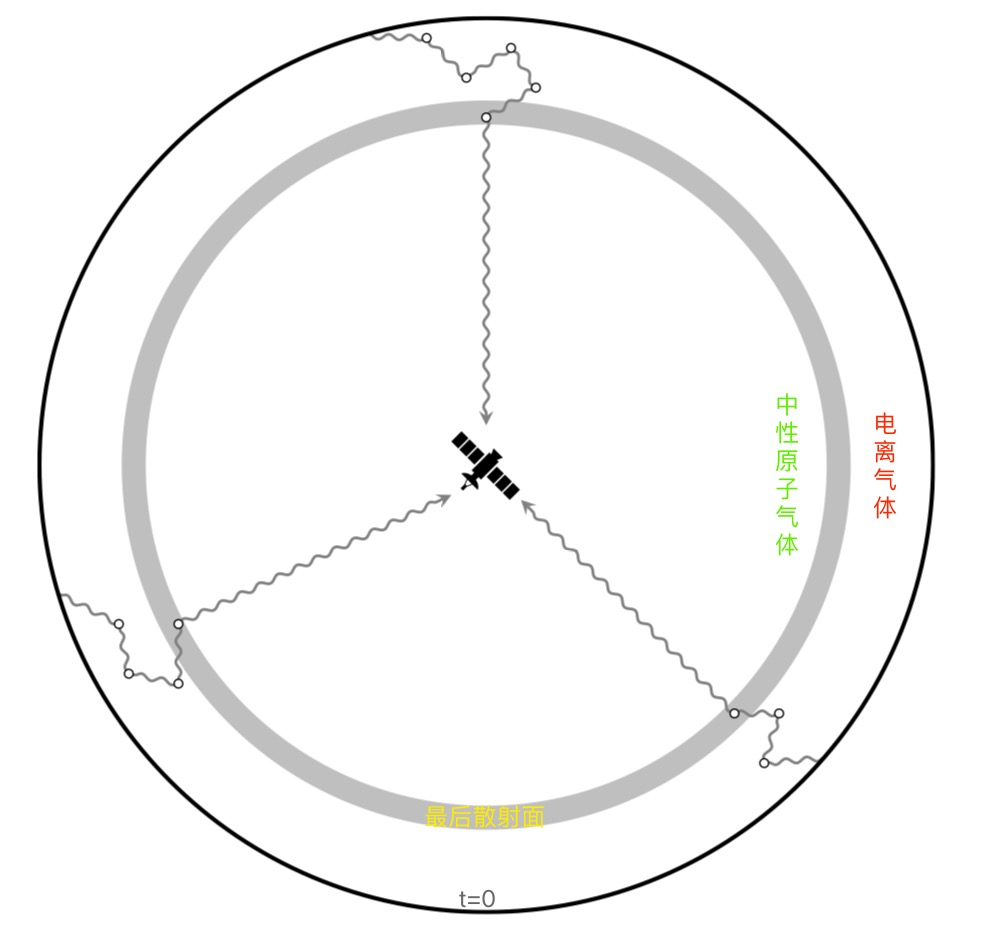
\includegraphics[width=1.0\linewidth]{lastScatter2022.jpg}
	\caption{图中灰色圆环为最后散射面,修改自 Daniel Baumann: Cosmology (2021)} \label{fig.LastScat}
\end{figure}

\subsection{CMB的特征}

\begin{itemize}
    \item 各向同性:来自所有方向的CMB温度高度相同。
    \item 辐射场强度随频率的分布符合黑体辐射谱。(Planck公式)
    \item 退耦能标约为 $0.3\mathrm{eV}$,温度约为3000K,红移约为1100
    \item 温度涨落有偶极矩。(因为地球、太阳、银河系的运动。)
    \item 扣除偶极矩后,仍然存在微小的温度起伏,这就是后来宇宙密度起伏、形成星系等结构的种子/初始条件。
\end{itemize}

为什么CMB符合黑体谱?

在最后散射面 $t_L$,光子辐射谱满足Planck公式:
\begin{equation}
    n_{T(t_L)}(\nu_L) d \nu_L=\frac{8 \pi \nu_L^{2} d \nu_L}{\exp \left(\frac{h_\text{pl} \nu_L}{k_{B} T(t_L)} \right)-1}
\end{equation}
在$t>t_L$,光子频率由于宇宙学红移降低 $\nu=\nu_{L} \frac{a(t_L)}{a(t)}$,
光子数密度 $n\left(\nu, t\right) d\nu \propto a^{-3}$即
\begin{equation}
    n(\nu, t) d \nu=\left(\frac{a(t_L)}{a(t)}\right)^{3} n_{T\left(t_{L}\right)}\left(\nu_{L}\right) d \nu_{L}
\end{equation}

代入得
\begin{equation}
    n(\nu, t) d \nu = \frac{8 \pi \nu^{2} d \nu}{\exp \left(\frac{h_\text{pl} \nu}{k_{B} \frac{a(t_L)}{a(t)}T(t_L)}   \right)-1}
\end{equation}
仍然是黑体谱。此时光子不处于热平衡,不妨令$T(t)=\frac{a(t_L)}{a(t)}T(t_L)$,即$T\propto 1/a$.

\end{document}
